\section{The Breakdown into Longer and Shorter Periods: the Years, Months, Days and Hours of Each Star. The Use of These Periods in Nativities.}

By taking one-twelfth of the year (or of each period) we can discover how many days each star/sign allots. For example: \Aries\xspace allots 15 years. One-twelfth of 15 years is 15 months. Next one-twelfth of 15 months is 37 1/2 days. Next one-twelfth of 37 1/2 days is 3 1/3 hours. <\Aries> allots these time-periods during its period of rule. The allotments of the other stars will be found in the same way. If anyone uses
this system, he will find the overall, the yearly, and the monthly chronocrators, as well as the daily and hourly chronocrators. We will append the time divisions for each star worked out in detail so as not to confuse \textbf{/170K/} our readers:\textbf{/161P/}

\clearpage
\begin{table}[ht]
\begin{center}
\caption{Planet Years, Months, Days, and Hours}
\label{Table 4.2}
\vspace{0.5cm}
\begin{tabular}{crrrc}
\toprule
\textbf{Star} & \textbf{Years} & \textbf{Months} & \textbf{Days} & \textbf{Days+Hours} \\
\midrule
\Sun & 19 & 19 & $47\frac{1}{2}$ & 3 days 23 hours \\
\Moon & 25 & 25 & $62\frac{1}{2}$ & 5 days 5 hours \\
\Saturn & 30 & 30 & 75 & 6 days 6 hours \\
\Capricorn & 27 & 27 & $67\frac{1}{2}$ & 5 days 15 hours \\
\Jupiter & 12 & 12 & 30 & 2 days 12 hours \\
\Mars & 15 & 15 & $37\frac{1}{2}$ & 3 days 3 hours \\
\Venus & 8 & 8 & 20 & 1 day 16 hours \\
\Mercury & 20 & 20 & 50 & 4 days 4 hours\\
\bottomrule
\end{tabular}
\end{center}
\end{table}

If we find a nativity it its 50th or 60th year, we begin the zodiacal vital sector of years from the Lot of Fortune or from Daimon, assigning to each star its period as far as it applies. Then we assign the months, then the day and hours. If the nativity is an infant’s, we begin by assigning the hours of the vital sector, then the days and months.

For example: \Sun, \Mercury, in \Capricorn, \Saturn, \Jupiter\xspace in \Leo, \Mars, \Venus\xspace in \Aquarius, \Moon\xspace in \Gemini, Ascendant in \Leo, the Lot of Fortune in \Pisces, the Lot of Daimon in \Capricorn
\footnote{\textit{Greek Horoscopes} dates the chart (L152) to approximately December 27, 152 AD (p.128)}. 

\clearpage
\begin{wrapfigure}[14]{R}{7cm}
\centering
\vspace{-20pt}
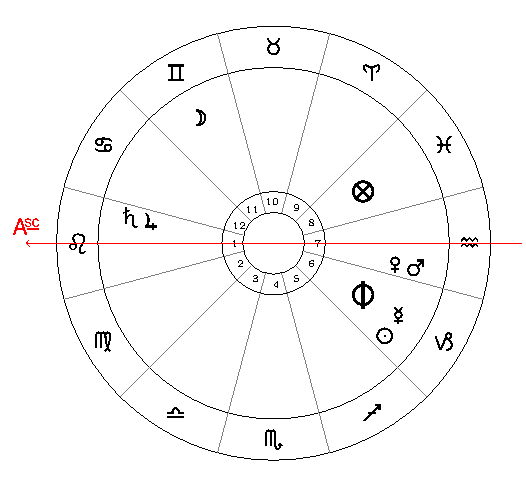
\includegraphics[width=0.68\textwidth]{charts/4_10_1}
\caption{Chart 52 [IV.10.1, GH L152]}
\label{fig:chart52}
\end{wrapfigure} 

Let the vital sector start at the Lot of Fortune in \Pisces. It is necessary to investigate the fourth year, Mesori 16,
including the 5 <intercalary> days of each year. Since 12 <years> for \Pisces would leave no allotment remaining, I have assigned 1 year <=12 months> to \Pisces, 1 year 3 month to \Aries, 8 months to \Taurus. The total so far is 2 years 11 months. Then the allotment passes to \Mercury, 1 year 8 months, to total 4 years 7 months. But the nativity has not yet completed this length of time, so let \Mercury\xspace be the chronocrator for a period of 8 months 15 days, a total of 255 days. It is necessary to allot this amount continuing <to count> in the order of the signs. First \Mercury\xspace gives to itself (i.e. to \Gemini) 50 days, then to \Cancer\xspace 62 1/2 days, then to \Leo\xspace 47 1/2 days, then to \Virgo\xspace 50 days, then to \Libra 20 days. The total so far is 230 days, with 25 remaining. 

Now \Mars will have these 25 days in \Scorpio\xspace after \Venus's days <in \Libra>, until the completion of 37 1/2 days. Therefore \Mars\xspace will allot the 25 days proceeding in the order of the signs. First it allots to itself 3 days 3 hours, then to \Sagittarius\xspace 2 1/2 days, then to
\Capricorn\xspace 5 days 15 hours, then to \Aquarius\xspace 6 days 6 hours, then to \Pisces\xspace 2 1/2 days, then to \Aries\xspace 3 days 3 hours, and to \Taurus\xspace the rest <1 day 21 hours> to complete the 25 days. 

The overall chronocrator is \Jupiter\xspace <\Pisces>; the second is \Mercury\xspace <\Gemini>, receiving the allotment from \Jupiter; the third is \Mars <\Scorpio>, receiving it from \Mercury; the fourth is \Venus <\Taurus>, receiving it \textbf{/171K/} from \Mars. For the nativity it will be necessary to examine \textbf{/162P/} where these stars are located and how they are configured with each other; having done this, then make your forecast\footnote{Riley: Some astrologers allot the days using the triangles - marginal note.}.

If the overall chronocrator is found to be a benefic, the \Sun, or the \Moon, it brings fame and leadership for the nativity, or prominent offices, benefits, and association with the great. 

In those chronocratorships when a malefic receives the distribution (according to the system of allotment), it brings about bodily infirmity and dangers. 

If another star which is in opposition to the overall chronocrator or is inappropriately configured at the nativity and in transit receives the days, it brings upset, anxieties, and penalties. 

If at the nativity the overall chronocrator happens to be unfavorably situated or is beheld by malefics, in the days assigned to those malefics the native will be ruined, fall into danger, or suffer crises. But if, when these malefics receive the chronocratorship, the overall chronocrator is found in operative signs and has benefics in aspect in transit, although embarrassed in livelihood or rank <during the period of the malefic>, the native will <later> live undisturbed.

In distributing the days, when you have completed the whole cycle of days (=528), it is necessary to begin the remaining days starting with the sign in opposition. In the same way for the lesser time-periods, i.e. the days and the hours—after the completion of the cycle of days and hours (=44), count off the
remaining days and hours in the order of the signs from the sign in opposition.

\newpage
